\documentclass[12pt]{article}

%Bibliography   
    \usepackage{apacite}
    \bibliographystyle{apacite}
    %http://www.ctan.org/tex-archive/biblio/bibtex/contrib/apacite/apacite.pdf
 
%Essay Header
	\pagestyle{myheadings}
	\markright{\hfill \emph{Horowitz }}

%pdfLaTeX: TeX Gyre Termes
	%\usepackage{tgtermes}
	\usepackage[T1]{fontenc}

%Sectioning
    \usepackage{sectsty}
    \sectionfont{\fontsize{13}{15}\selectfont}

%Packages
    \usepackage[margin=1in]{geometry}
    \usepackage{setspace}
    \usepackage[leftmargin = 1in, rightmargin = 0in, vskip = 0in]{quoting}
    \usepackage{microtype}




\newtoggle{professormode}
%\toggletrue{professormode} %STUDENTS: DELETE or COMMENT this line



\title{MATH 390.4 Spring 2020 Homework \#5}

\author{Tziporah Horowitz} %STUDENTS: write your name here

\iftoggle{professormode}{
\date{Due Monday, May 18, 2020 11:59PM by email\\ \vspace{0.5cm} \small (this document last updated \currenttime~on \today)}
}

\renewcommand{\abstractname}{Instructions and Philosophy}

\begin{document}
\maketitle


\iftoggle{professormode}{
\begin{abstract}
The path to success in this class is to do many problems. Unlike other courses, exclusively doing reading(s) will not help. Coming to lecture is akin to watching workout videos; thinking about and solving problems on your own is the actual ``working out.''  Feel free to \qu{work out} with others; \textbf{I want you to work on this in groups.}

Reading is still \textit{required}. For this homework set, you should finish Silver's book but I am not asking any questions on ch12, 13 and the conclusion. They are very interesting though! You should be googling and reading about all the concepts introduced in class online. This is your responsibility to supplement in-class with \textit{your own} readings.

The problems below are color coded: \ingreen{green} problems are considered \textit{easy} and marked \qu{[easy]}; \inorange{yellow} problems are considered \textit{intermediate} and marked \qu{[harder]}, \inred{red} problems are considered \textit{difficult} and marked \qu{[difficult]} and \inpurple{purple} problems are extra credit. The \textit{easy} problems are intended to be ``giveaways'' if you went to class. Do as much as you can of the others; I expect you to at least attempt the \textit{difficult} problems. 

This homework is worth 100 points but the point distribution will not be determined until after the due date. See syllabus for the policy on late homework.

Up to 7 points are given as a bonus if the homework is typed using \LaTeX. Links to instaling \LaTeX~and program for compiling \LaTeX~is found on the syllabus. You are encouraged to use \url{overleaf.com}. If you are handing in homework this way, read the comments in the code; there are two lines to comment out and you should replace my name with yours and write your section. The easiest way to use overleaf is to copy the raw text from hwxx.tex and preamble.tex into two new overleaf tex files with the same name. If you are asked to make drawings, you can take a picture of your handwritten drawing and insert them as figures or leave space using the \qu{$\backslash$vspace} command and draw them in after printing or attach them stapled.

The document is available with spaces for you to write your answers. If not using \LaTeX, print this document \textit{including this first page} and write in your answers. \inred{I do not accept homeworks which are \textit{not} on this printout.}

\end{abstract}

\thispagestyle{empty}
\vspace{1cm}
NAME: \line(1,0){380}
\clearpage
}



%\problem{These are questions about the rest of Silver's book: ch12, 13 and the conclusion. For all parts in this question, answer using notation from class (i.e. $t ,f, g, h^*, \delta, \epsilon, e, t, z_1, \ldots, z_t, \mathbb{D}, \mathcal{H}, \mathcal{A}, \mathcal{X}$, $\mathcal{Y}, X, y, n, p, x_{\cdot 1}, \ldots, x_{\cdot p}$, $x_{1 \cdot}, \ldots, x_{n \cdot}$, etc.) as well as in-class concepts (e.g. simulation, validation, overfitting, etc.)}
%
%\begin{enumerate}
%
%\easysubproblem{}\spc{1}
%
%\end{enumerate}

\section{The CART Algorithms}

\begin{enumerate}
\easysubproblem{Write down the step-by-step $\mathcal{A}$ for regression trees.
\ans Let the dataset be all the data,
\begin{enumerate}
    \item Consider every possible orthogonal-to-axis split ($X_j \leq X_{ij} \ \forall \ j = 1, \ldots, p, \\
    i \in \{1, \ldots, n-1\}$). Compute $SSE_l$ and $SSE_r$ (the $SEE$'s in the left node and the right node). Select the node where $SSE_{weighted} = \frac{n_l SSE_l + n_r SSE_r}{n_l + n_r}$ is the smallest, i.e. create an inner node with that split rule, a left leaf with $\yhat = \ybar_l$, and a right leaf with $\yhat = \ybar_r$.
    \item If $n_l > N_0$ (a hyperparameter), set the dataset on the left of the partition and run (a) on it. If $n_r > N_0$, set the dataset on the right of the partition and run (a) on it.
\end{enumerate}
}

\hardsubproblem{Describe $\mathcal{H}$ for regression trees. This is very difficult but doable. If you can't get it in mathematical form, describe it as best as you can in English.
\ans $\mathcal{H}$ is the set of all split rules.
}

\intermediatesubproblem{Think of another \qu{leaf assignment} rule besides the average of the responses in the node that makes sense.
\ans \begin{align*}
    \yhat = \text{Median}[\y]
\end{align*}
}

\intermediatesubproblem{Assume the $y$ values are unique in $\mathbb{D}$. Imagine if $N_0 = 1$ so that each leaf gets one observation and its $\yhat = y_i$ (where $i$ denotes the number of the observation that lands in the leaf) and thus it's very overfit and needs to be \qu{regularized}. Write up an algorithm that finds the optimal tree by pruning one node at a time iteratively. \qu{Prune} means to identify an inner node whose daughter nodes are both leaves and deleting both daughter nodes and converting the inner node into a leaf whose $\yhat$ becomes the average of the responses in the observations that were in the deleted daughter nodes. This is an example of a \qu{backwards stepwise procedure} i.e. the iterations transition from more complex to less complex models.
\ans \begin{enumerate}
    \item Determine the OOSE of the initial tree.
    \item Compute the OSSE for each possible pruning and retain the tree with the lowest error.
    \item Repeat (b) until the OOSE begins to increase.
\end{enumerate}
}


\hardsubproblem{Provide an example of an $f(\x)$ relationship with medium noise $\delta$ where vanilla OLS would beat regression trees in oos predictive accuracy. Hint: this is a trick question.
\ans If $f(\x)$ is a linear equation, OLS will be able to model it with low error.
\begin{align*}
    f(\x) = b_0 + b_1x_1 + \ldots + b_px_p
\end{align*}
}

\easysubproblem{Write down the step-by-step $\mathcal{A}$ for classification trees. Feel free to reference steps in (a).
\ans \begin{enumerate}
    \item Consider every possible orthogonal-to-axis split ($X_j \leq X_{ij}\ \forall \ j= 1,\ldots,p, \\ i \in \{1, \ldots, n-1\}$). Rather than selecting the node where $SSE_{weighted}$ is the smallest, select the node where $Gini_N = \frac{n_l Gini_l + n_r Gini_r}{n_l + n_r}$  is the smallest, where  $Gini_l = \sum_{k=1}^k \hat{p}_k(1-\hat{p}_k)$ and $\hat{p}_k = \sum_{i=1}^{n_l} \indic_{y_i = c_k}$. Leaf assignment will be based on the mode instead of the mean.
    \item Same as step (b) in question (a).
\end{enumerate}
}

\hardsubproblem{Think of another objective function that makes sense besides the Gini that can be used to compare the \qu{quality} of splits within inner nodes of a classification tree.
\ans Calculate the Information Gain of each split.
}


\end{enumerate}

\section{Probability Estimation and \\ Asymmetric Cost Modeling}

\begin{enumerate}
\easysubproblem{Why is logistic regression an example of a \qu{generalized linear model} (glm)?
\ans Because we retain $\vect{w} \cdot \x$ in the hypothesis set.
}

\easysubproblem{What is $\mathcal{H}_{pr}$ for the probability estimation algorithm that employs the linear model in the covariates with logistic link function?
\ans \begin{align*}
    \mathcal{H}_{pr} = \bigg\{\oneover{1 + e^{-\vect{w} \cdot \x}} : \vect{w} \in \reals^{p+1} \bigg\}
\end{align*}
}

\easysubproblem{If logistic regression predicts 3.1415 for a new $\x_*$, what is the probability estimate that $y=1$ for this $\x_*$?
\ans \begin{align*}
    p \approx 1
\end{align*}
}

\intermediatesubproblem{What is $\mathcal{H}_{pr}$ for the probability estimation algorithm that employs the linear model in the covariates with cloglog link function?
\ans \begin{align*}
    \mathcal{H}_{pr} = \big\{1 - e^{-e^{\vect{w} \cdot \x}} : \vect{w} \in \reals^{p+1} \big\}
\end{align*}
}

\hardsubproblem{Generalize linear probability estimation to the case where $\mathcal{Y} = \braces{C_1, C_2, C_3}$. Use the logistic link function like in logistic regression. Write down the objective function that you would numerically maximize. This objective function is one that is argmax'd over the parameters (you define what these parameters are --- that is part of the question). 

Once you get the answer you can see how this easily goes to $K > 3$ response categories. The algorithm for general $K$ is known as \qu{multinomial logistic regression}, \qu{polytomous LR}, \qu{multiclass LR}, \qu{softmax regression}, \qu{multinomial logit} (mlogit), the \qu{maximum entropy} (MaxEnt) classifier, and the \qu{conditional maximum entropy model}. You can inflate your resume with lots of jazz by doing this one question!
\ans \begin{align*}
    \argmax_{\vect{w} \in \reals^{p+1}} \bigg\{ \oneover{1 + \sum e^{-\vect{w} \cdot \x}} \bigg\}
\end{align*}
}

\easysubproblem{Graph a canonical ROC and label the axes. In your drawing estimate AUC. Explain very clearly what is measured by the $x$ axis and the $y$ axis.
\ans \begin{center}
    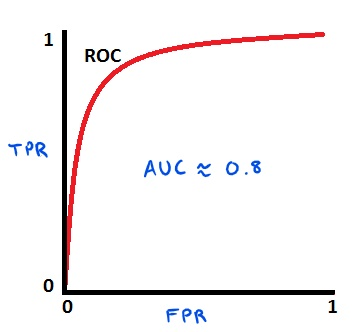
\includegraphics[scale = 0.5]{roc 1.jpg}
\end{center}
FPR is the rate at which negatives are discovered as false positives. TPR is the rate at which positives are discovered as true positives.

}

\easysubproblem{Pick one point on your ROC curve from the previous question. Explain a situation why you would employ this model.
\ans \begin{center}
    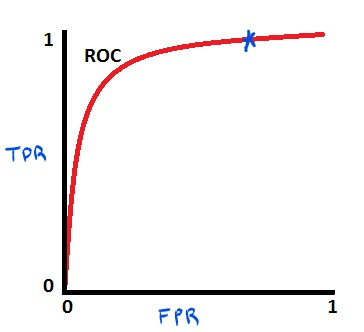
\includegraphics[scale = 0.5]{roc 2.jpg}
\end{center}
We care more about the reward of predicting true negatives than the cost of a false positives.
}


\easysubproblem{Graph a canonical DET curve and label the axes. Explain very clearly what is measured by the $x$ axis and the $y$ axis.
\ans \begin{center}
    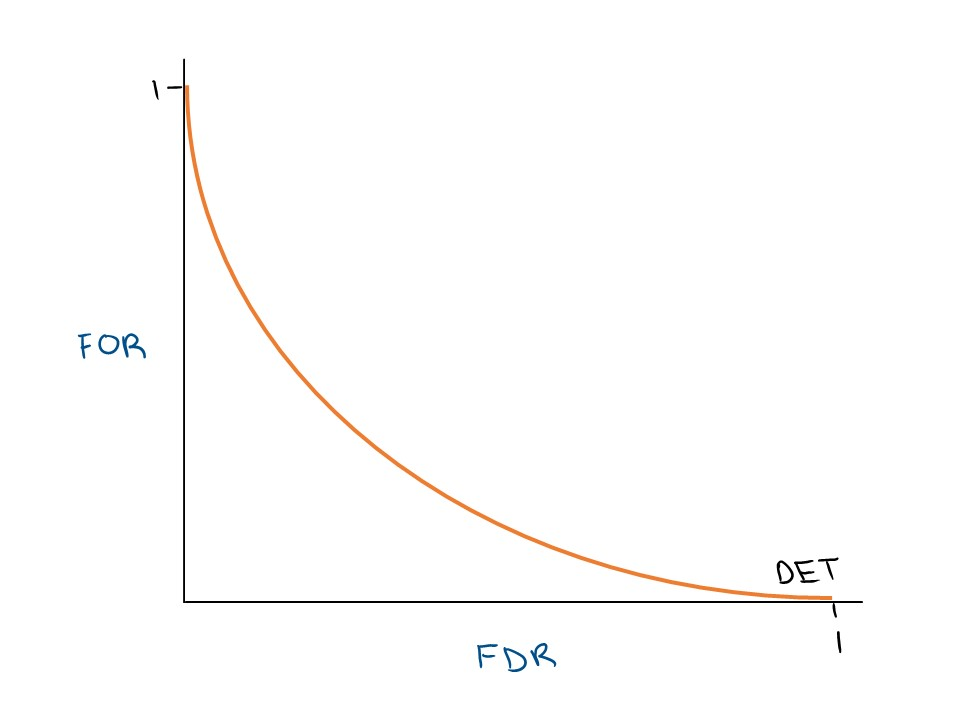
\includegraphics[scale = 0.3]{det 1.jpg}
\end{center}
FDR is the proportion of discovered positives that are false. FOR is the proportion of discovered negatives that are false.
}

\pagebreak

\easysubproblem{Pick one point on your DET curve from the previous question. Explain a situation why you would employ this model.
\ans \begin{center}
    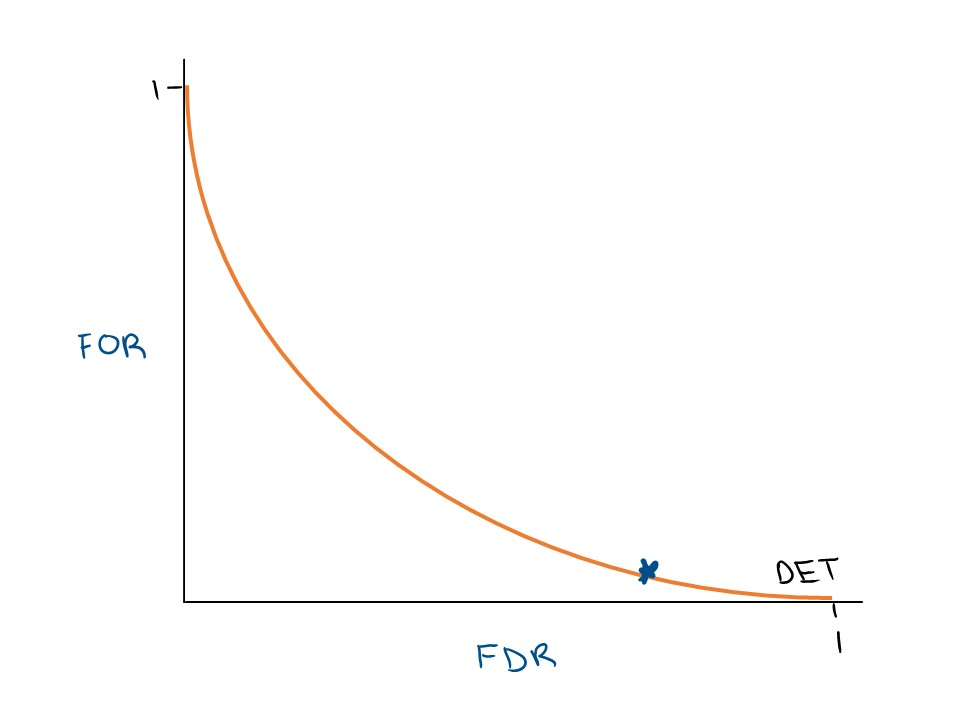
\includegraphics[scale = 0.3]{det 2.jpg}
\end{center}
We care more about the cost of a false negative than the cost of a false positive.
}

\hardsubproblem{The line of random guessing on the ROC curve is the diagonal line with slope one extending from the origin. What is the corresponding line of random guessing in the DET curve? This is not easy...
\ans The line of random guessing on the DET curve would be the diagonal line with the $y$ intercept of 1 and the slope -1.
}
\end{enumerate}


\section{Bias-Variance Decomposition}
Assume the two assumptions from the notes about the random variable model that produces the $\delta$ values, the error due to ignorance.

\begin{enumerate}
\easysubproblem{Write down (do not derive) the decomposition of MSE for a given $\x_*$ where $\mathbb{D}$ is assumed fixed but the response associated with $\x_*$ is assumed random.
\ans \begin{align*}
    MSE(\x_*) = \sigsq + \big(f(\x_*) - g(\x_*) \big)^2
\end{align*}
}

\easysubproblem{Write down (do not derive) the decomposition of MSE for a given $\x_*$ where the responses in $\mathbb{D}$ is random but the $\X$ matrix is assumed fixed and the response associated with $\x_*$ is assumed random like previously.
\ans \begin{align*}
    MSE(\x_*) = \sigsq + \text{Bias}[G]^2 + \var{G}
\end{align*}
}

\easysubproblem{Write down (do not derive) the decomposition of MSE for general predictions of a phenomenon where all quantities are considered random.
\ans \begin{align*}
    MSE = \sigsq + \expe{\text{Bias}[G]^2} + \expe{\var{G}}
\end{align*}
}

\hardsubproblem{Why is it in (a) there is only a \qu{bias} but no \qu{variance} term? Why did the additional source of randomness in (b) spawn the variance term, a new source of error?
\ans There is no variance term in (a) because there is only one model. In (b), the randomness in $\mathbb{D}$ creates different $\delta$'s so there is variance in the distribution of multiple models.
}

\intermediatesubproblem{A high bias / low variance algorithm is underfit or overfit?
\ans Underfit.
}

\intermediatesubproblem{A low bias / high variance algorithm is underfit or overfit?
\ans Overfit.
}

\intermediatesubproblem{Explain why bagging reduces MSE for \qu{free} regardless of the algorithm employed.
\ans It allows $\mathcal{H}$ to be very expressive, so the Bias$[g_i]$ is approximately 0 for all $i$.
}

\intermediatesubproblem{Explain why RF reduces MSE atop bagging $M$ trees and specifically mention the target that it attacks in the MSE decomposition formula and why it's able to reduce that target.
\ans Since bagging reduces the bias to approximately 0, 
\begin{align*}
    MSE \approx \sigsq + \rho \expe{\var{g_{(m)}}}
\end{align*}
where $\rho$ is the average correlation between two trees. Random Forest attacks $\rho$ by splitting on a subset of features of size $p_{try} < p$ after node construction, thereby making the trees more different from one another.
}

\hardsubproblem{When can RF lose to bagging $M$ trees? Hint: setting this critical hyperparameter too low will do the trick.
\ans If the hyperparameter is too low, the bias will increase too much.
}
\end{enumerate}

\section{Lasso, Ridge, and the Elastic Net}

\begin{enumerate}
\easysubproblem{Write down the objective function to be minimized for ridge. Use $\lambda$ as the hyperparameter.
\ans \begin{align*}
    \vect{b} = \argmin_{\vect{w} \in \reals^{p+1}} \big\{ SSE + \lambda || \vect{w} ||^2 \big\}
\end{align*}
}

\easysubproblem{Write down the objective function to be minimized for lasso. Use $\lambda$ as the hyperparameter.
\ans \begin{align*}
    \vect{b} = \argmin_{\vect{w} \in \reals^{p+1}} \big\{ SSE + \lambda || \vect{w} || \big\}
\end{align*}
}

\easysubproblem{We spoke in class about when ridge and lasso are employed. Based on this discussion, why should we restrict $\lambda > 0$?
\ans If $\lambda = 0$, $\X^\top \X$ is not invertable. If $\lambda < 0$, $\vect{b}$ can be 0.
}

\intermediatesubproblem{Why is lasso sometimes used a preprocessing step to remove variables that likely are not important in predicting the response?
\ans Lasso sets many elements of $\vect{b}$ to 0.
}


\easysubproblem{Assume $\X$ is orthonormal. One can derive $\b_{\text{lasso}}$ in closed form. Copy the answer from the wikipedia page. Compare $\b_{\text{lasso}}$ to $\b_{\text{OLS}}$.
\ans \begin{align*}
    \vect{\hat{\beta}} = (\X^\top \X)^{-1} \X^{\top} \y \cdot \text{max}\bigg(0, 1 - \frac{N\lambda}{|(\X^\top \X)^{-1} \X^{\top} \y|} \bigg)
\end{align*}
}

\intermediatesubproblem{Write down the objective function to be minimized for the elastic net. Use $\alpha$ and $\lambda$ as the hyperparameters.
\ans \begin{align*}
    \vect{b} = \argmin_{\vect{w} \in \reals^{p+1}} \Big\{SSE + \lambda \big(\alpha ||\vect{w}||_1 + (1 - \alpha) ||\vect{w}||_2^2 \big) \Big\}
\end{align*}
}

\easysubproblem{We spoke in class about the concept of the elastic net. Based on this discussion, why should we restrict $\alpha \in (0, 1)$?
\ans So that both ridge and lasso will be factored into the regression.
}

\end{enumerate}


\section{Missingness}

\begin{enumerate}
\easysubproblem{What are the three missing data mechanisms? Provide an example when each occurs (i.e., a real world situation).
\ans \begin{itemize}
    \item \emph{Missing Completely at Random} (MCAR). Ex: there are random missing values in the data that have nothing to do with one another. 
    \item \emph{Missing at Random} (MAR). Ex: Men are more likely to report their weight than women.
    \item \emph{Not Missing at Random} (NMAR). Ex: retired seniors not filling out hourly wage in a survey.
\end{itemize}
}

\easysubproblem{Why is listwise-deletion a terrible idea to employ in your $\mathbb{D}$ when doing supervised learning?
\ans You can end up dropping too much important data.
}

\easysubproblem{Why is it good practice to augment $\mathbb{D}$ to include missingness dummies? In other words, why would this increase oos predictive accuracy?
\ans The dummy variables take the weight of the missing data.
}

\easysubproblem{To impute missing values in $\mathbb{D}$, what is a good default strategy and why?
\ans Use missForest because it guarantees convergence of the imputed values.
}

\end{enumerate}


\section{Correlation-Causation and \\ Interpretation of OLS coefficients.}

\begin{enumerate}
\easysubproblem{Consider a fitted OLS model for y with features $x_1$, $x_2$, \ldots, $x_p$. Provide the most correct interpretation of the quantity $b_1$ you can.
\ans When computing two "mutually observed" independent observations A and B, sampled in the same fashion as observations in $\mathbb{D}$, when A has an $x_1$ measurement one unit larger than B's $x_1$ measurement but both A and B share the same features $x_1, \ldots, x_p$ then A is predicted to have a response $y$ that differs on average by $b_1$ units from the response $y$ of B.
}


\easysubproblem{If $x$ and $y$ are correlated but their relationship isn't causal, draw a diagram below that includes $z$.
\ans \begin{center}
    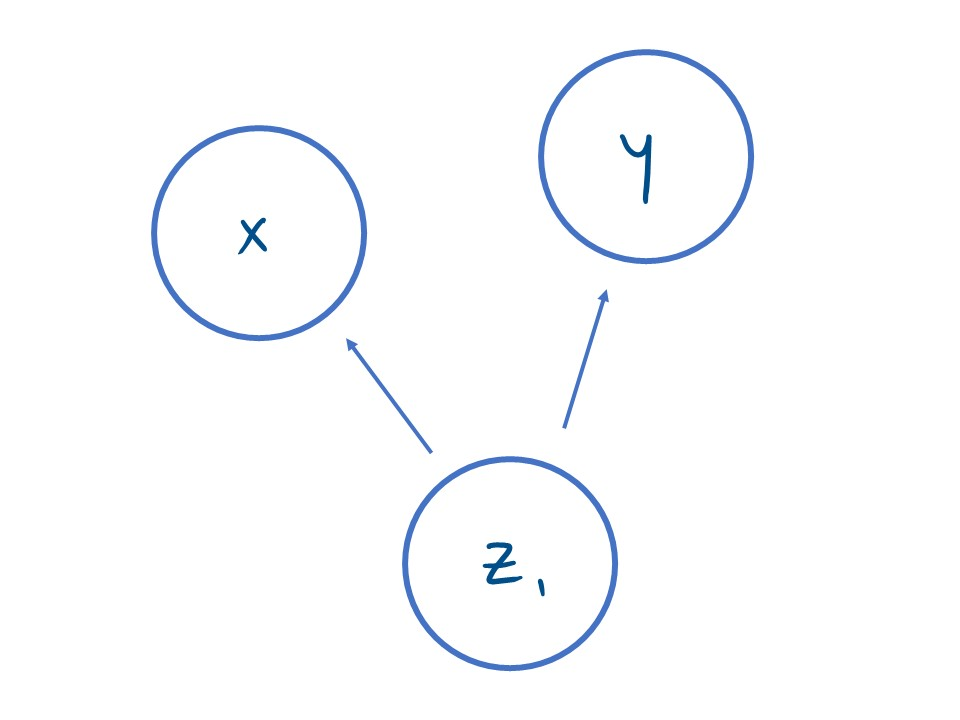
\includegraphics[scale = 0.3]{corr not cause.jpg}
\end{center}
}

\easysubproblem{To show that $x$ is causal for $y$, what specifically has to be demonstrated? Answer with a couple of sentences.
\ans To have a causal relationship, $x$ must be connected to $y$, whether directly or indirectly. Often in modeling, the causal relationship is indirect, i.e. $x$ causes $z$ and $z$ causes $y$ along with other factors.
}

\intermediatesubproblem{If we fit a model for y using $x_1$, $x_2$, \ldots, $x_7$, provide an example real-world illustration of the causal diagram for $y$ including the $z_1$, $z_2$, $z_3$.
\ans \begin{center}
    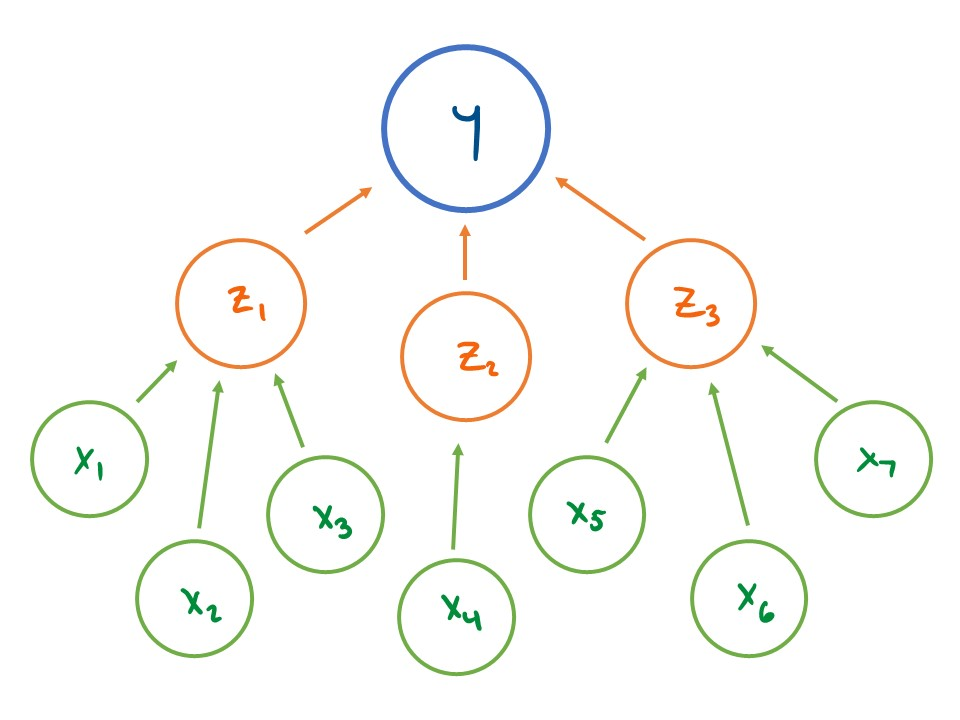
\includegraphics[scale = 0.35]{cause.jpg}
\end{center}
}


\end{enumerate}

\end{document}
